\subsubsection{Teilausfall bei der Haupt-API}

Bei einem Teilausfall der Haupt-API hat die Docker-Compose-Umgebung es bei keinem Testdurchlauf geschafft, den Service innerhalb des Testfensters selbst wiederherzustellen, wie in der Tabelle \ref{tab:chaos_api_instance_down} zu sehen ist.
Dadurch hat Docker keinen der Tests bestanden, weshalb der Zuverlässigkeits-Score der Docker-Compose-Umgebung bei jeder Testumgebung eine 0 beträgt, wie in Abbildung \ref{fig:chaos_api_instance_down} zu sehen ist. 
Die k3s-Umgebung hat dagegen jeweils einen Score von 60 Punkten oder mehr erzielt.
Zur Wiederherstellung des Services hat k3s im Durchschnitt weniger als eine Sekunde gebraucht. Da die Docker-Compose-Umgebung den Service nicht von selbst wiederherstellen konnte, wurde keine Zeit eingetragen, da diese nur die Länge vom Chaos-Anfang bis Testende betragen würde. 
\begin{table}[htbp]
\centering
\caption{Vergleich der Chaos-Test-Metriken bei Teilausfall der Haupt-API}
\label{tab:chaos_api_instance_down}

\begin{tabular}{lrr}
\toprule
\textbf{Metrik} & \textbf{Docker} & \textbf{K3s} \\
\midrule
Error Rate [\%]         & 98.96 & 3.11 \\
Availability [\%]       & 1.04 & 96.89 \\
Recovery Time [s]      & - & 0.44 \\
Recovered [Anzahl]      & 0 & 3 \\
\bottomrule
\end{tabular}

\end{table}

\begin{figure}[htbp]
\centering
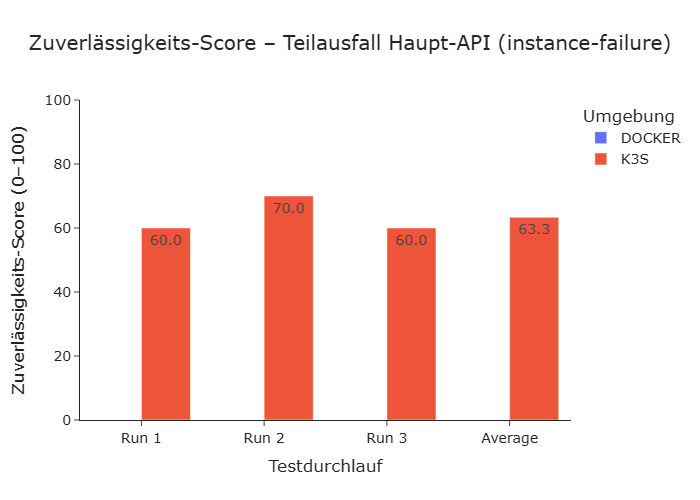
\includegraphics[width=0.8\textwidth]{bilder/tests/reliability_score_api-instance-down_instance-failure.png}
\caption{Zuverlässigkeit Score bei Teilausfall der Haupt-API}
\label{fig:chaos_api_instance_down}
\end{figure}
\FloatBarrier